%\documentclass[3p,preprint]{elsarticle}
\documentclass[3p,twocolumn]{elsarticle}

\usepackage[colorlinks,citecolor=blue]{hyperref}
%\usepackage{lineno}
%\modulolinenumbers[5]
\usepackage{amsmath}
\usepackage{amssymb}
\usepackage[]{natbib}
\usepackage[version=4]{mhchem}
\usepackage{adjustbox}   
\usepackage[position=top,captionskip=0pt]{subfig}
\usepackage{graphicx}
\DeclareGraphicsExtensions{.pdf,.eps,.png}

\usepackage{xcolor}
\usepackage{pdfcomment}

\newcommand{\diff}[2]{\dfrac{\partial #1}{\partial #2}}

\journal{Fluid Phase Equilibria}

\bibliographystyle{elsarticle-num}
%%%%%%%%%%%%%%%%%%%%%%%

\begin{document}

\begin{frontmatter}

\title{A molecular dynamics study of the solvation of carbon dioxide and other compounds in the ionic liquids \ce{[emim][B(CN)_4]} and \ce{[emim][NTf_2]}}
%\title{A molecular dynamics study of the solvation of \ce{CO_2}, \ce{H_2O}, and some organic compounds in the ionic liquids \ce{[emim][B(CN)_4]} and \ce{[emim][NTf_2]}}

%% Group authors per affiliation:
\author[plapiqui]{A.J.~Silveira\corref{curradd}}
\author[plapiqui]{S.~Pereda}
\author[eq-ufrj,coppe-ufrj]{F.W.~Tavares}
\author[eq-ufrj]{C.R.A.~Abreu\corref{cor1}}
\ead{abreu@eq.ufrj.br}

\address[plapiqui]{Planta Piloto de Ingenier\'ia Qu\'imica (PLAPIQUI), Universidad Nacional del Sur, Bah\'ia Blanca, Argentina}
\address[eq-ufrj]{Chemical Engineering Department, Escola de Qu\'imica, Universidade Federal do Rio de Janeiro, Rio de Janeiro, Brazil}
\address[coppe-ufrj]{Chemical Engineering Program, Alberto Luiz Coimbra Institute for Graduate Studies and Research in Engineering (COPPE), Universidade Federal do Rio de Janeiro, Rio de Janeiro, Brazil}

\cortext[curradd]{Current address: Computational \& Systems Biology Program, Memorial Sloan Kettering Cancer Center, New York, NY, USA}
\cortext[cor1]{Corresponding author}

\begin{abstract}
In this paper, we calculate solvation free energies of several compounds in ionic liquids.
These free energies are used to compute properties such as Henry's law constants and activity coefficients, generally required in the design of environmentally sustainable processes.
It is known, for instance, that carbon dioxide from combustion is one of the main sources of anthropogenic greenhouse gases.
Recently, the propensity of the ionic liquid \ce{[emim][B(CN)_4]} for the physisorption of \ce{CO_2} has been reported, which makes it a potential solvent for carbon capture.
In the present work, molecular dynamics simulations of the solvation of \ce{CO_2} in ionic liquids \ce{[emim][B(CN)_4]} and \ce{[emim][NTf_2]} are carried out both at infinite dilution and at high concentrations.
A systematic study is performed by comparing several force fields and assessing the efficacy of simplification measures such as rigid-body dynamics and pairwise electrostatics.
Our results confirm recent experimental observations that, for a given volume of solvent, lower pressure is required to absorb a certain amount of \ce{CO_2} in \ce{[emim][B(CN)_4]} than in other ionic liquids.
\end{abstract}

\begin{keyword}
ionic liquids \sep solvation free energy \sep \ce{CO_2} Henry's law constant \sep infinite-dilution activity coefficient
\end{keyword}

\end{frontmatter}

%\linenumbers

\section{Introduction}
\label{sec:intro}

\ce{CO_2} emissions from fossil-fuel power generation plants account for a large portion of the anthropogenic greenhouse gases \cite{totalenergy}.
International efforts aimed at regulating and reducing \ce{CO_2} emissions are increasing \cite{Tong_2018} and, in this context, the development of technologies for the capture and storage of \ce{CO_2} plays an essential role \cite{Markewitz_2014}.

The conventional process for \ce{CO_2} removal comprises a chemical absorption followed by stripping at high temperatures.
The most commonly used solvents are volatile organic compounds, specially aqueous solutions of monoethanolamine (MEA).
Despite its high absorption capability, the use of MEA has a serious drawback, which is the high cost of solvent recovery \cite{Merkel_2010}.
Other disadvantages include corrosion and degradation by oxidation, as well as solvent loss by evaporation.
The latter also contributes to the increase of environmental pollution and generates extra costs for replacing the solvent.

The use of ionic liquids (ILs) as solvents for \ce{CO_2} sequestration receives special attention in the investigation of alternative technologies.
The reasons are their well-known properties such as almost negligible vapor pressure and high thermal stability.
Furthermore, they are particularly attractive since they can be designed for specific applications, giving rise to the so-called task-specific ILs \cite{Seo_2014}.
These remarkable properties make ILs suitable for a wide variety of applications in separation processes \cite{Han_2010,Werner_2010}, catalysis \cite{P_rvulescu_2007}, energy management \cite{MacFarlane_2014}, and material science \cite{Mecerreyes_2011,Tom_2015,Dupont_2010,Leones_2017,Kinik_2017}.

Recently, Carvalho \textit{et al}. \cite{Carvalho_2016} called into question the potentiality of ILs for \ce{CO_2} capture.
They warn that the use of molar fraction to express solubility has, to some extent, perpetuated misconceptions regarding the supposedly high absorption capability of certain ILs.
Although most thermodynamic models are formulated in terms of molar fractions, a key factor that dictates the efficiency of absorption process  is given by the amount of \ce{CO_2} that can be dissolved in a certain \textit{volume} or \textit{mass} of solvent.
By expressing the solubility values in terms of molality and performing an exhaustive comparison among various ILs, Carvalho \textit{et al}. \cite{Carvalho_2016} show that most systems which promote physical absorption of \ce{CO_2} exhibit solubilities which are similar, or even lower, than that observed for heavy alkanes such as eicosane.
This is true for the popular ILs \ce{[bmim][NTf_2]}, \ce{[bmim][PF_6]}, \ce{[bmim][BF_4]}, as well as for those synthesized from the fluorination of the cation or the anion, such as \ce{[(C_2H_2F_2)mim][NTf_2]} and \ce{[hmim][pFAP]}.
The only exception they found was the family of ILs containing the anion \ce{[B(CN)_4]^-} (tetracyanoborate).

There is no obvious explanation accounting for the enhanced solubility promoted by the presence of \ce{[B(CN)_4]^-}.
In this context, molecular simulation provides us with a powerful tool for studying solvation processes.
To the best of our knowledge, only one study in the literature reports computation of solvation free energy for \ce{CO_2} in \ce{[emim][B(CN)_4]} by molecular simulation \cite{Liu_2014_1}.
Nonetheless, the computed value is overestimated, as observed by deriving a Henry's law constant and comparing it to available experimental data.
Such scarcity motivated us to carry out the present investigation, in which we have evaluated different force fields for \ce{[emim][B(CN)_4]} proposed in the literature.
As we show here, it was possible to find a model that successfully reproduces the experimental value of the Henry constant of \ce{CO_2} in this IL.
For comparison, we analyzed the solvation of \ce{CO_2} not only in \ce{[emim][B(CN)_4]}, but also in \ce{[emim][NTf_2]}, both at infinite dilution and at high concentrations.
The simulations confirmed what is observed in experiments.
For \ce{[emim][B(CN)_4]}, a considerably lower pressure is required to dissolve the same amount of \ce{CO_2}, considering a given mass of solvent.
In addition, we also calculated infinite-dilution activity coefficients of other solutes in \ce{[emim][B(CN)_4]} and compared the results with experimental values recently reported in literature.
The solutes we considered were hexane, benzene, cyclohexane, ethanol, and water.

This paper is organized as follows.
In Sec.~\ref{sec:theory}, we present the theoretical background of this work, which is followed by a brief description of the employed force fields in Sec.~\ref{sec:force_field}.
The methodological details are provided in Sec.~\ref{sec:sim_details}, while the corresponding numerical results are given in Sec.~\ref{sec:results}.
Finally, we present some concluding remarks in Sec.~\ref{sec:conclusion}.

\section{Theoretical background}
\label{sec:theory}

In this section, we present the formalism that allows us to compute solvation free energies from molecular dynamics simulations and, after that, to obtain Henry constants and activity coefficients.
For dealing with systems at infinite dilution at low pressures, we rely on the work of Shirts \textit{et al}. \cite{Shirts_2003}.
Then, we reformulate the equations in order to study concentrated solutions and systems at higher pressures, which is a more likely scenario in the case of \ce{CO_2} capture processes.

\subsection*{Solvation Free Energy}

The solvation free energy, $\Delta G_{\text{solv}}$, is defined as the reversible work needed to transfer a solute molecule from a gas phase to a liquid solution.
For dense systems, an efficient computation of solvation properties via molecular simulation is possible by means of the so-called alchemical methods, which employ non-physical pathways to reversibly connect the endpoint states whose difference in free energy is to be estimated.
In the case of $\Delta G_{\text{solv}}$, the alchemical route involves a gradual insertion/deletion of the solute through the definition of a coupling parameter $\lambda$, which scales the solute-solvent interactions by taking values in the interval [0,1]. By convention, $\lambda = 1$ corresponds to a fully interacting system, while for $\lambda$ = 0 the solute-solvent interactions are turned off completely.

In what follows, the subscripts ``s'' and ``IL'' refer to the solute and the solvent (ionic liquid), respectively.
For a liquid phase containing $N_\text{IL}$ solvent molecules and $N_{\text{s}}$ solute molecules at fixed pressure (P) and temperature (T), the difference in free energy between the states associated to $\lambda$ = 1 and $\lambda$ = 0 is formally defined as
\begin{equation}
\Delta G_\text{sim} \equiv R T \ln \frac{\Xi (N_s,N_\text{IL},P,T,\lambda = 1)}{\Xi (N_s,N_\text{IL},P,T,\lambda = 0)}, 
\end{equation}
where $\Xi$ denotes the isobaric-isothermal partition function and $R$ is the gas constant.
Shirts \textit{et al}. \cite{Shirts_2003} rigorously derived the working expression that relates $\Delta G_\text{sim}$ to what is experimentally measured as the solvation free energy, namely
\begin{equation}
\label{eq:solvation free energy definition}
\Delta G_{\text{solv}} \equiv R T \ln \left( \frac{P_s}{c_s R T} \right),
\end{equation}
where $P_s$ is the partial pressure of the solute in the gas phase and
$c_s$ is the molar concentration of the solute in the liquid phase.
Note that these quantities correspond to a phase equilibrium condition.
For obtaining the mentioned relation, the authors derived an expression for the chemical potential of the solute in the liquid phase ($\mu^l_s$) as a function of $\Delta G_\text{sim}$, which can be written as
\begin{equation}
\label{eq:solute chemical potential}
\mu^l_s = \mu^{ig}_s + \Delta G_\text{sim} - RT \ln \left( \frac{V^{\ast}}{V_1}\right) - RT \ln \left( \frac{P_s}{c_s R T} \right),
\end{equation}
where $\mu^{ig}_s$ is the chemical potential of the solute in an ideal gas at temperature $T$ and solute partial pressure $P_s$, while $V^{\ast}$ and $V_1$ are the mean volumes of liquid solutions specified by ($N_s-1$,$N_\text{IL}$,P,T) and ($N_s$,$N_\text{IL}$,P,T), respectively.
Note that $c_s = \frac{N_s}{N_A V_1}$, where $N_A$ is the Avogadro number.

Finally, by treating the gas phase as an ideal gas and considering the system to be at equilibrium ($\mu^l_s = \mu^{ig}_s$), Shirts \textit{et al}. \cite{Shirts_2003} found out that
\begin{equation}
\begin{split}
\label{eq:free_solv}
 \Delta G_{\text{solv}} = \Delta G_\text{sim} - RT \ln \left( \frac{V^{\ast}}{V_1}\right).
\end{split}
\end{equation}

For small solutes, such as those considered in this work, the term containing the ratio $V^{\ast}/V_1$ is typically in the order of magnitude of the free-energy uncertainties \cite{Shirts_2003}.
Hence, it can be neglected and will be omitted hereafter.

\subsection*{Henry's Law Constant}

If both $P_s$ and $c_s$ are small, we can resort to Eqs.~\eqref{eq:solvation free energy definition} and \eqref{eq:free_solv} to predict Henry's law constant, which is defined as $\text{K}_s =\frac{P_s}{x_s}$ \cite{Prausnitz}.
%\begin{equation}
%\text{K}_s =\frac{P_s}{x_s}.
%\end{equation}
%
Therefore, by simply expressing Eq.~\eqref{eq:solvation free energy definition} in terms of the molar fraction of the solute in the liquid phase ($x_s$), we can conclude that
\begin{equation}
\label{eq:henry_eq}
K_s = \tilde{\rho}_\text{sim} R \, T \exp\left(\frac{\Delta G_\text{sim}}{R T}\right),
\end{equation}
where $\tilde{\rho}_\text{sim}$ is the simulated molar density of the solution. Assuming that this solution is very dilute, one can use the molar density of pure solvent ($\tilde{\rho}_\text{IL}$) instead.

\subsection*{Higher Pressure Conditions}
\label{sec:partial_pressure}

For the ILs of interest to the present investigation, high concentrations of \ce{CO_2} in the liquid phase are obtained at pressure values for which, in principle, the ideal gas assumption might no longer be valid.
In this case, we can compute the chemical potential of the solute in the real gas phase as
\begin{equation}
\label{eq:mu_gas_real}
\mu^{g}_s = \mu^{ig}_s + R T \ln \left(\frac{f^{g}_s}{P_s}\right),
\end{equation}
where $f^{g}_s$ is the fugacity of the solute in the gas phase.
Then, by considering a system at phase equilibrium ($\mu^{l}_s$ = $\mu^{g}_s$), it follows that
\begin{equation}
\label{eq:fgas_d}
f^{g}_s = c_s R T \exp \left( \frac{\Delta G_\text{sim}}{R T} \right). 
\end{equation}

Three additional assumptions are made here. First, we assume that the gas phase is either pure solute (which is consistent with the ionic-liquid systems with which we compare our simulations) or can be approximated by an ideal solution. Second, we assume that the system pressure is moderate, so that a truncated virial equation is enough to represent the gas phase. In this case, Eq.~\eqref{eq:fgas_d} becomes
\begin{equation}
\label{eq:equilibrium pressure}
y_s \exp\left( \frac{B_s P}{R T} \right) P = c_s R T \exp \left( \frac{\Delta G_\text{sim}}{R T} \right),
\end{equation}
where $y_s$ is the molar fraction of solute in the gas phase ($y_s \rightarrow 1$ for the systems we analyze here) and $B_s$ is the second virial coefficient of the solute.
In the case of \ce{CO_2}, we employ the correlation for $B_s$ developed by Holste \textit{et al}. \cite{Holste_1987}, which is
\begin{equation}
B_s = B_0 + \frac{B_1}{T} + \frac{B_2}{T^2},
\end{equation}
where $B_0 = 23.02991~\mathrm{\frac{cm^3}{mol}}$, $B_1 = -2455.297~\mathrm{\frac{K \cdot cm^3}{mol}}$, and $B_2 = -1.22675 \times 10^7~\mathrm{\frac{K^2 \cdot cm^3}{mol}}$.

Our third assumption, supported by preliminary simulations, is that $\Delta G_\text{sim}$ does not vary appreciably with pressure, at least over the range of experimental data considered here.
In this way, no iterative simulations are required to compute the equilibrium pressure when solving Eq.~\eqref{eq:equilibrium pressure} for $P$.

\subsection*{Activity Coefficients}

As will be shown below, the prediction of activity coefficients requires additional simulations of the solute as a pure liquid phase, whose properties we denote here by a superscript ``$0$''.
We start by using a standard thermodynamic relation \cite{Tester} to write the solute activity coefficient $\gamma_s$ in terms of chemical potentials as
\begin{equation}
\label{eq:gamma}
\ln \gamma_s = \frac{\mu_s^l - \mu_s^{l,0}}{R T} - \ln x_s,
\end{equation}

Next, we replace $\mu_s^l$ and $\mu_s^{l,0}$ by their corresponding instances of Eq.~\eqref{eq:solute chemical potential}. In this step, we note that $c_s = \tilde{\rho} x_s$ and $c_s^0 = \tilde{\rho}_s^0$, where $\tilde{\rho}$ and $\tilde{\rho}_s^0$ are the molar densities of the solution and of pure liquid solute, respectively. Thus, the expression we obtain for computing an activity coefficient from two independent simulations is
\begin{equation}
\ln \gamma_s = \frac{\Delta G_\text{sim} - \Delta G_\text{sim}^{0}}{R T} + \ln \frac{\tilde{\rho}}{\tilde{\rho}_s^0}.
\end{equation}

In the special case of a solute at infinite dilution in an ionic liquid solvent, its activity coefficient $\gamma^\infty_s$ can be computed by replacing $\tilde{\rho}$ in the equation above by the molar density of the pure solvent, $\tilde{\rho}_\textit{IL}$.

\section{Force fields}
\label{sec:force_field}

\subsection{Ionic liquids}
\label{sec:force_field_il}

The versatility of ILs for different applications is in part due to the fact that their physical properties strongly depend on the particular cation-anion combination.
On the other hand, this feature also explains why the desirable transferability of force fields is particularly difficult to attain.
Indeed, it is a common practice to extract the potential parameters of the intramolecular (bond stretching, angle bending, torsion rotation) and Lennard-Jones (LJ) interactions from a well established force field and, then, only derive the partial atomic charges with the aim of adjusting the model for a specific pair of ions.
This procedure is, however, inconsistent with conventional force field parameterization in which the determination of atomic charges precedes the establishment of torsional terms.
Another ad-hoc strategy, which intends to roughly incorporate polarization effects, is to scale the partial charges uniformly with a factor which normally takes values in the range from 0.8 to 0.9.
This has proven to be effective for predicting dynamic properties \cite{Schr_der_2012}.

In this paper, we analyze four different models for \ce{[emim][B(CN)_4]}.
Koller \textit{et al}. \cite{Koller_2012} were the first to introduce a specific non-polarizable force field for this IL.
They tested three variations of a united-atoms model, in which the hydrogen atoms of alkyl groups \ce{CH_3} and \ce{CH_2} of cation \ce{[emim]^+} are treated implicitly.
Among these variations, the one named FF-3 best reproduces the experimental values of density, self-diffusion coefficients, and viscosity.
In short, Koller \textit{et al}. \cite{Koller_2012} took both the intramolecular and LJ parameters for the cation from the work of Liu \textit{et al}. \cite{Liu_2006}, which in turn based their model on the AMBER \cite{Cornell_1995} framework.
The intramolecular parameters involving the boron atom were extracted from the DREIDING \cite{Mayo_1990} force field and the anionic van der Waals parameters were refined based on the values reported by Price \textit{et al}. \cite{Price_2001}.
The atomic partial charges were derived using the EA-RESP method \cite{Basma_2001} from Post-Hartree-Fock \textit{ab-initio} calculations at MP2/6-31G\textsuperscript{*}+ level of theory, which automatically resulted in total charges on the ions of $\pm0.8426~\mathrm{e}$.

Batista \textit{et al}. \cite{Batista_2015} then used the parameters of Ref.~\citenum{Koller_2012} for \ce{[B(CN)_4]^-} to study aqueous solutions of \ce{[emim][B(CN)_4]}.
In this case, the authors considered the all-atom model of Cadena and Maginn \cite{Cadena_2006} for \ce{[emim]^+}.
The atomic partial charges were obtained using the CHELP procedure \cite{Breneman_1990}, resulting in net charges of $\pm 0.889~\mathrm{e}$.
It should be noted that the factors for scaling the 1-4 non-bonded interactions are different for these force fields.
Cadena and Maginn \cite{Cadena_2006} apply factors of 1.0 and 0.4 for the LJ and Coulombic interactions, respectively, while for Koller \textit{et al}. \cite{Koller_2012} the corresponding values are 1/2 and 5/6, in accordance with the AMBER force field.
Batista \textit{et al}. \cite{Batista_2015} used the former throughout (J. Coutinho, personal communication).

Another set of parameters for \ce{[emim][B(CN)_4]} was derived by Liu \textit{et al}. \cite{Liu_2014} in a study that investigates the dynamics of \ce{CO_2} and \ce{N_2} dissolved in this ionic liquid.
Parameters corresponding to the intramolecular and LJ interactions were extracted from GAFF \cite{Wang_2004}, while the atomic partial charges were computed using the RESP method \cite{Bayly_1993} with B3LYP/6-311+G(d) DFT calculations.
The net charges of the ions were manually adjusted to $\pm 0.8 ~\mathrm{e}$.

Finally, we also consider the parameterization which Weber and Kirchner \cite{Weber_2016} carried out for \ce{[emim][B(CN)_4]} based on the force field developed by P{\'{a}}dua and Canongia Lopes \cite{Canongia_Lopes_2006}.
As the potential parameters for the anion were specified neither in Ref.~\citenum{Weber_2016} nor in Ref.~\citenum{Canongia_Lopes_2006}, we obtained them by direct communication with the authors of Ref.~\citenum{Weber_2016}.
The atomic partial charges were derived using the RESP procedure with Hartree-Fock calculations at the \mbox{6-31++G\textsuperscript{**}} level of theory, resulting in net charges of $\pm 0.8 ~\mathrm{e}$.

In the case of ionic liquid \ce{[emim][NTf_2]}, we use the model of K\"{o}ddermann \textit{et al}. \cite{Koddermann_2007}, which was also derived by refining parameters of the force field by P{\'{a}}dua and Canongia Lopes \cite{Canongia_Lopes_2006}.
The authors characterized this refinement as unusual, given that they modified the LJ parameters while keeping the partial charges unchanged.
Kerl \textit{et al}. \cite{Kerl__2017} recently employed this model to accurately predict Henry constants of \ce{CO_2} in \ce{[emim][NTf_2]} at several temperatures.

\subsection{Solutes}
\label{sec:force_field_sol}

Besides \ce{CO_2}, the solutes considered in this work are hexane, benzene, ethanol, cyclohexane, and water.
Hexane and benzene were modeled using the OPLS-AA force field \cite{Jorgensen_1996}, while the TRAPPE potential \cite{Chen_2001,Potoff_2001} was employed for ethanol and \ce{CO_2}.
Cyclohexane was simulated using a rigid-body model \cite{munoz2015lennard} whose sites interact via a LJ potential only.
For water, we employ the TIP4P/2005 model \cite{Abascal_2005,Vega_2011}.

\section{Computational methods}
\label{sec:sim_details}

With the aim of setting up a computationally efficient protocol for the IL simulations, in this work we assess the possibilities of modeling the ions as rigid bodies and employing the damped shifted force (DSF) method \cite{Fennell2006} for computing electrostatic interactions.
In this method, the electrostatic potential between two atoms with charges $q_i$ and $q_j$ interacting at a distance $r$ is given by
\begin{equation}
V_\text{DSF}(r) = V(r) - V(r_c) - V^\prime(r_c)(r-r_c),
\end{equation}
where $V(r) = q_i q_j {\text{erfc}(\alpha r)}/{r}$ is a damped Coulomb potential.
This potential is cut off at $r = r_c$, which makes it short-ranged and thus a cheaper alternative to Ewald-type schemes \cite{Ewald_1921,Darden_1993,Hockney_1988}.
McCann \textit{et al}. \cite{McCann_2013} tested the DSF method for various ILs modeled with the OPLS-AA force field.
They concluded that using $\alpha = 0.2~\text{\AA}^{-1}$ and $r_c = 15~\text{\AA}$ provides the best energetic agreement with the Ewald method.
In this work, detailed comparisons are made in terms of the simulated densities and radial distribution functions.
In Sec.~\ref{sec:results}, we show that by using the same $\alpha$ value but a considerably smaller cutoff distance ($r_c = 12 \text{\AA}$) one can obtain suitable results.
These values were employed here for the ILs as well as for solutes containing partially charged atoms.
The only exception was hexane, for which the use of undamped Coulombic interactions (i.e. $\alpha = 0$) resulted in improved chemical potential predictions.

The NPT algorithm of Kamberaj \textit{et al}. \cite{Kamberaj_2005} was used to integrate the equations of motion for rigid bodies.
For flexible molecules, we applied the integration scheme of Shinoda \textit{et al}. \cite{Shinoda2004}, with the lengths of all C-H bonds constrained by the SHAKE method \cite{Ryckaert1977}.
For both integrators, we used a small time-step size ($\Delta t$) of 1 fs in order to avoid discretization-induced artifacts \cite{Eastwood_2010, Silveira_2017}.

The gradual insertion/deletion of solutes involves scaling both the van der Waals (vdW) and the electrostatic intermolecular interactions.
To avoid numerical instabilities associated to the vdW scaling, it is usual to employ a soft-core potential with nonlinear coupling.
In this paper, we use the modified LJ potential proposed by Beutler \textit{et al}. \cite{Beutler_1994}, given by $V_\text{vdW}(r) = 4 \epsilon \lambda_\text{vdW} (s^{-2} - s^{-1})$, where $s = (r/\sigma)^6 + (1 - \lambda_\text{vdW})/2$.
The electrostatic interactions, on the other hand, can be linearly scaled by a coupling parameter $\lambda_\text{Coul}$ \cite{Naden_2015}, meaning that $V_\text{Coul}(r) = \lambda_\text{Coul} V_\text{DSF}(r)$.
Furthermore, the vdW and Coulomb contributions to the free energy difference are taken into account separately.
That is,
\begin{equation}
\Delta G_\text{sim} = \Delta G_\text{vdW} + \Delta G_\text{Coul},
\end{equation}
where $\Delta G_\text{vdW}$ is computed by varying $\lambda_\text{vdW} \in [0,1]$ while keeping $\lambda_\text{Coul} = 0$, whereas $\Delta G_\text{Coul}$ is computed by varying $\lambda_\text{Coul} \in [0,1]$ while keeping $\lambda_\text{vdW} = 1$.
The sets of coupling parameter values we use here in all alchemical simulations are $\lambda_{\text{vdW}}$ = $\{0.0$, $0.05$, $0.1$, $0.2$, $0.25$, $0.3$, $0.35$, $0.4$, $0.45$, $0.5$, $0.6$, $0.7$, $0.8$, $0.9$, $1.0\}$ and $\lambda_{\text{Coul}}$ = $\{0.0$, $0.1$, $0.4$, $0.7$, $0.1\}$.

In this work, we compute $\Delta G_\text{Coul}$ by carrying out an independent simulation of 10 ns at each state of $\lambda_{\text{Coul}}$.
In the end, we apply the Multistate Bennett Acceptance Ratio (MBAR) method \cite{Shirts_2008} by using the \textit{Alchemical Analysis} package \cite{Klimovich_2015}.

In the case of $\Delta G_\text{vdW}$, the Expanded Ensemble method \cite{Lyubartsev_1992} is applied for sampling the whole $\lambda_\text{vdW}$ set in a single simulation.
An expanded ensemble is constructed as a weighted sum of subensembles, each one assuming a different value of the parameter selected for exploring the free energy landscape, which in our case is $\lambda_\text{vdW}$.
In the method adopted here \cite{Chodera_2011_2}, simulating an expanded ensemble comprises doing molecular dynamics (MD) at fixed N, P, T, and $\lambda_\text{vdW}$ amid Monte Carlo (MC) transitions in the value of $\lambda_\text{vdW}$.
The number of MD steps between transitions is fixed and, at each transition, one of the $\lambda_\text{vdW}$ states is picked at random according to a corresponding set of probabilities \cite{Chodera_2011_2}.
In addition, a set of biasing weights is included in the MC acceptance criterion, thus making it possible to enhance the sampling procedure by iteratively tuning these weights until all $\lambda_\text{vdW}$ states are visited with equal frequency \cite{Lyubartsev_1992}.
Given that sample decorrelation is improved by having short MD runs between MC transitions \cite{Chodera_2011_2}, we used only 5 steps in each run.
In the iteration process for tuning the biasing weights, the simulation times for the preliminary and the final expanded ensemble rounds are 10 and 40 ns, respectively.
In this way, 3 iterations were sufficient in all cases for attaining, in the final round, an acceptable uncertainty in $\Delta G_\text{sim}$ estimated via MBAR \cite{Shirts_2008, Klimovich_2015}.

We first carried out MD simulations of isolated ion pairs in order to obtain minimum-energy conformations.
For this, we used a Nos\'{e}-Hoover chain thermostat \cite{Martyna1992} with set-point temperature gradually changing down to nearly $0~\text{K}$.
The resulting coordinates were then used with the PACKMOL algorithm \cite{Mart_nez_2009} via the Playmol package \cite{playmol} to obtain initial liquid-phase configurations.
The expanded ensemble procedure, the softcore potential, and the DSF method  with linear coupling were implemented by customizing the LAMMPS package \cite{Plimpton1995}, which we used for carrying out all the simulations in this work.

\section{Results and Discussion}
\label{sec:results}

\subsection{Ionic-Liquid Simulation Strategies}
\label{sec:prel_results}

In this section, we analyze the possibility of introducing simplifications in the molecular modeling and simulation of ionic liquids without substantially affecting the resulting thermodynamics properties.
For this, we compare results obtained with a \textit{standard} methodology to those obtained with a \textit{simplified} one.
The standard setup comprises simulating ions with moving bonds, angles, and dihedrals and using the Particle-Particle/Particle-Mesh (PPPM) Ewald method \cite{Hockney_1988} for calculating the Coulomb interactions.
In this case, a real-space cutoff of $12~\text{\AA}$ and a tolerance of $10^{-4}$ are used in LAMMPS for automatic determination of PPPM parameters such as damping factor and FFT grid spacing.
In the simplified setup, the ions are modeled as rigid bodies and the DSF method \cite{Fennell2006} with $r_c = 12 ~\text{\AA}$ and $\alpha = 0.2 ~\text{\AA}^{-1}$) is used as and alternative to the PPPM scheme.
For building the rigid bodies, we carry out a frequency analysis of some key dihedrals present in ions \ce{[emim]^+} and \ce{[NTf_2]^-}, whose flexibility could lead to significant conformational changes.
On the other hand, small and highly symmetric anions such as \ce{PF_6} and \ce{BF_4} are already usually modeled as rigid bodies \cite{HANKE_2001,Hanke_2003,Lynden_Bell_2006}, which justifies the strategy in the case of \ce{[B(CN)_4]^-}.

As a guide to the discussions in this section, in Fig~\ref{fig:atoms_id} we introduce a nomenclature for all atoms present in the ions \ce{[emim]^+}, \ce{[B(CN)_4]^-}, and \ce{[NTf_2]^-}.
Please note that, in the united-atom version of \ce{[emim]^+}, all hydrogen atoms ranging from H4 to H11 are incorporated to their corresponding carbon atoms.

\begin{figure}
\centering
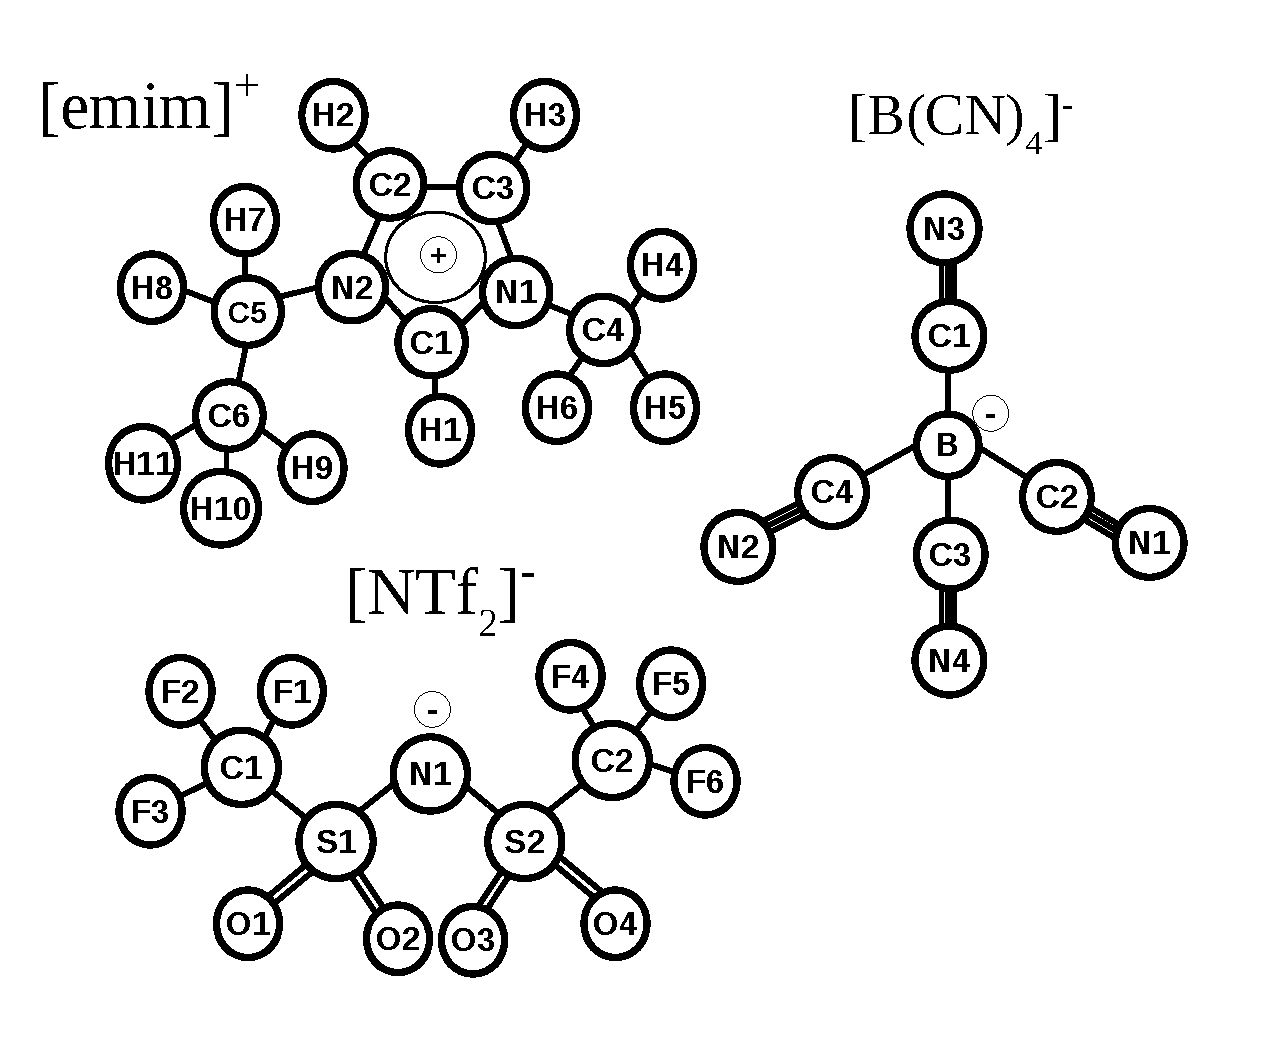
\includegraphics[width=\linewidth]{atoms_id.pdf}
\caption{Adopted nomenclature for individual atoms in the cation 1-ethyl-3-methylimidazolium (\ce{[emim]^+}) and anions tetracyano borate (\ce{[B(CN)_4]^-}) and bis(trifluoromethylsulfonyl)amide (\ce{[NTf_2]^-}).}
\label{fig:atoms_id}
\end{figure}

Using the software TRAVIS \cite{Brehm_2011}, we obtained combined distribution functions (CDFs) of the dihedral angles formed in \ce{[emim]^+} by atoms C1-N2-C5-C6 and atoms C2-N2-C5-C6.
These angles will be referred to as $\psi_1$ and $\psi_2$, respectively.
In Fig.~\ref{fig:dihedrals_emim}, we show the CDFs obtained for all force fields employed here for \ce{[emim][B(CN)_4]}.
All CDFs shown in this section were generated from NPT-MD simulations of 250 ion pairs at $T = 298.0~\mathrm{K}$ and $P = 1.0~\mathrm{bar}$ using our standard setup (i.e. flexible ions with PPPM Ewald electrostatics).
Initial inspection reveals that, in all cases, $\psi_1$ and $\psi_2$ populate regions of the diagrams around the two straight lines given by
\begin{equation}
\label{eq:dihedral angles}
\psi_2 = \begin{cases}
\psi_1 + 180^\circ & \text{if} \quad \psi_1 \leq 180^\circ \\
\psi_1 - 180^\circ & \text{if} \quad \psi_1 > 180^\circ
\end{cases},
\end{equation}
both corresponding to a coplanar structure formed by atoms C1, C2, N2, and C5.
%There are two such lines in each diagram because atom C6 can be located on either side of the plane.
One can note in Fig.~\ref{fig:dihedrals_emim} that the CDF peaks, which indicate the most likely dihedral angle combinations, lie either precisely above these lines or very close to them.
The largest distortions from coplanarity occur for the Batista \textit{et al}. \cite{Batista_2015} model, as observed by the peak locations in Fig.~\ref{fig:dihedrals_emim}(b).
Despite this, all rigid bodies considered here for \ce{[emim]^+} are built in such a way that atoms C[1-5], H[1-3], and N[1-2] all lie in a single plane.
Therefore, for specifying the torsion of bond N2-C5 it is enough to set a value for $\psi_1$ and then compute $\psi_2$ by means of Eq.~\eqref{eq:dihedral angles}.
All other structural features (bond lengths, bending angles, and hydrogen-involving dihedrals) are taken from the minimum-energy structure obtained for each force field.

One can note in Figs.~\ref{fig:dihedrals_emim}(a) and \ref{fig:dihedrals_emim}(c) that the Koller \textit{et al}. \cite{Koller_2012} and Liu \textit{et al}. \cite{Liu_2014} models display a very similar, orderly behavior with regard to the torsion angles.
The similarity is not surprising since both models are based on the AMBER framework \cite{Cornell_1995}.
In both diagrams, the most likely angle combinations can be found in narrow regions around $\psi_1 = 90^\circ$ and $\psi_1 = 270^\circ$.
These angles correspond to similar configurations (imagine, for instance, the effect of rotating the whole cation around the axis defined by bond N2-C5).
Hence, we decided to build a single rigid-body structure with $\psi_1 = 90^\circ$ for the united-atom version of \ce{[emim]^+}, which is the model of Koller \textit{et al}. \cite{Koller_2012}.
In the case of the all-atom model of Liu \textit{et al}. \cite{Liu_2014}, we considered a system composed by equal amounts of two rigid-body structures with $\psi_1 = 90^\circ$ and $\psi_1 = 270^\circ$.
For the Batista \textit{et al}. \cite{Batista_2015} model, once again we took the most likely values of $\psi_1$ ($102.6^\circ$ and $257.4^\circ$) so as to build two types of rigid bodies and consider them in equal amounts.
Finally, given the wide ranges of likely angle combinations in the case of the Weber and Kirchner model \cite{Weber_2016}, as observed in Fig.~\ref{fig:dihedrals_emim}(d), we defined four types of rigid bodies in this case.
The $\psi_1$-angle values for these types are $0^\circ$, $150^\circ$, $180^\circ$, and $210^\circ$, while their fractions in the system are 15\%, 30\%, 25\%, and 30\%, respectively.

\begin{figure*}
\centering
\subfloat[][Koller~\textit{et al}.~\cite{Koller_2012}]{
  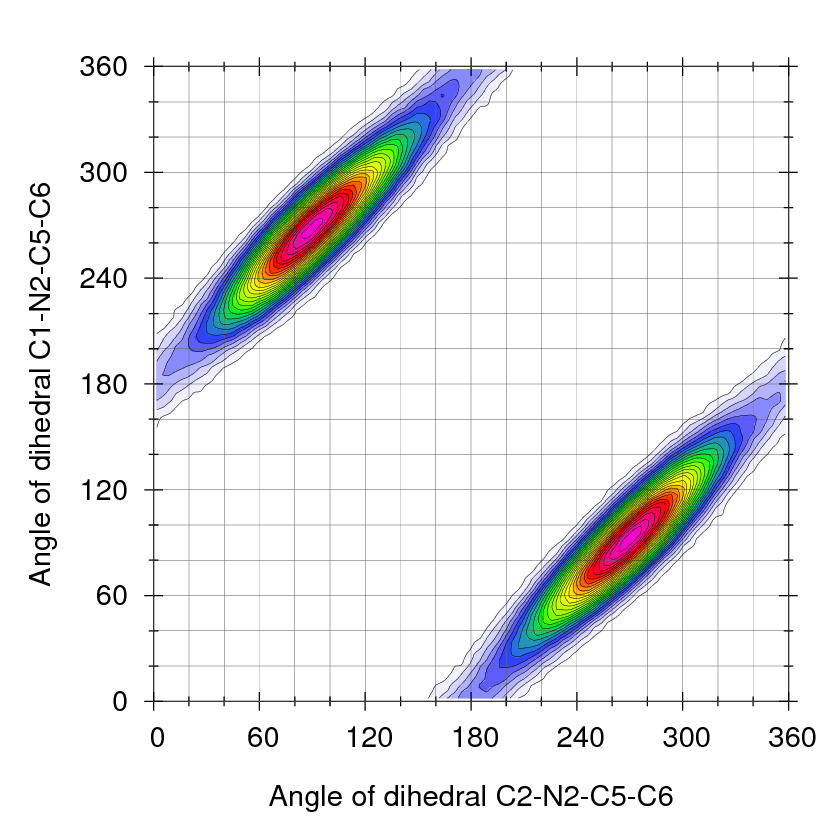
\includegraphics[width=.4\linewidth,trim={0 0 0 12pt},clip]{koller}}
\subfloat[Batista~\textit{et al}.~\cite{Batista_2015}]{  
  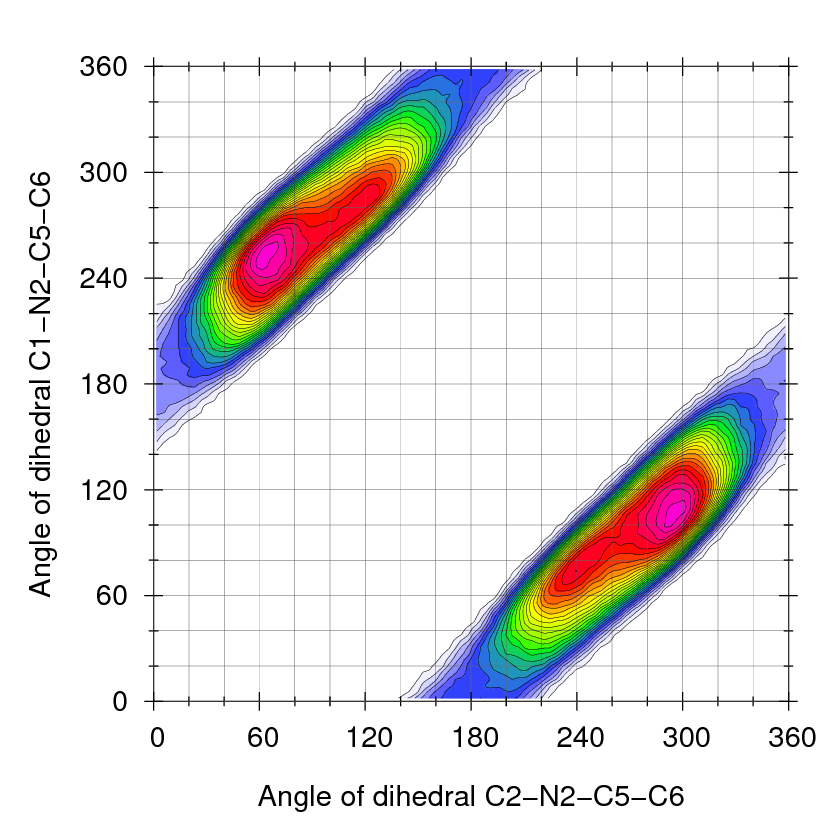
\includegraphics[width=.4\linewidth,trim={0 0 0 12pt},clip]{batista}}

\subfloat[Liu~\textit{et al}.~\cite{Liu_2014}]{%
  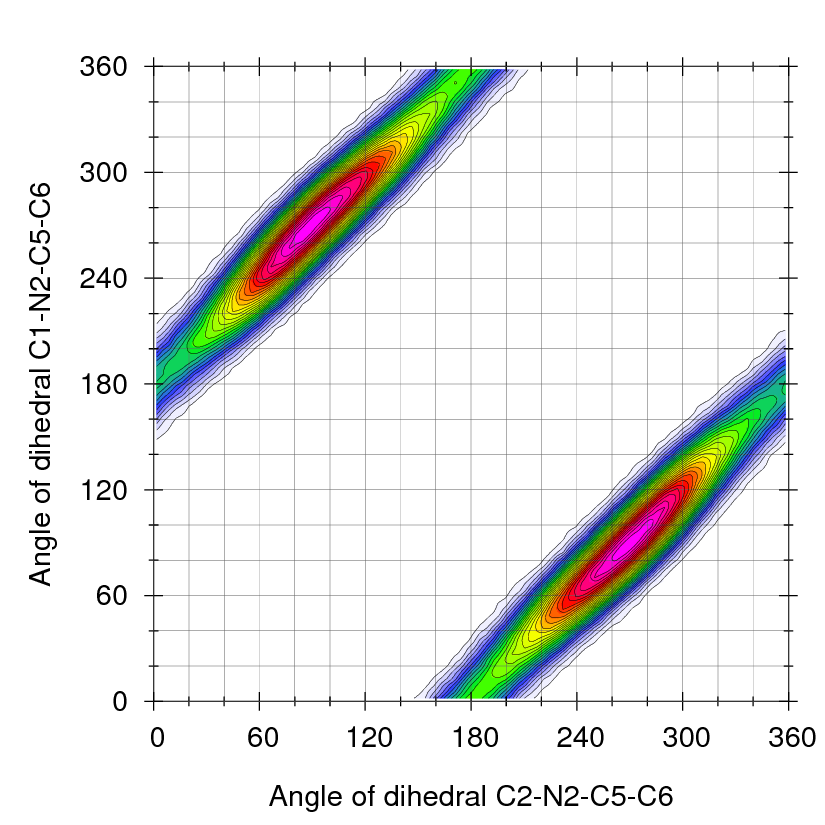
\includegraphics[width=.4\linewidth,trim={0 0 0 12pt},clip]{Liu}}%
\subfloat[Weber and Kirchner~\cite{Weber_2016}]{%
  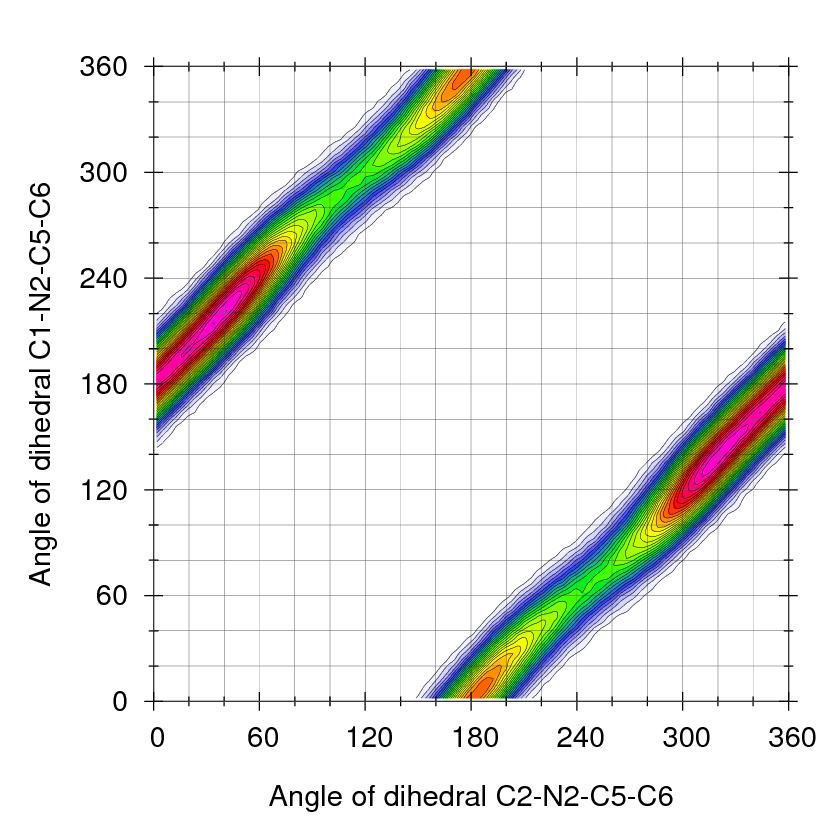
\includegraphics[width=.4\linewidth,trim={0 0 0 12pt},clip]{Weber}}%
\caption{Combined distribution functions of the dihedral angles corresponding to atoms C1-N2-C5-C6 and C2-N2-C5-C6 in the cation \ce{[emim]^+} (see Fig.~\ref{fig:atoms_id}), as sampled in NPT-MD simulations of 250 ion pairs using each model for \ce{[emim][B(CN)_4]}.}
\label{fig:dihedrals_emim}
\end{figure*}

Once the rigid body structures have been determined, we carried out NPT-MD simulations of 250 ion pairs at $T = 298.0~\mathrm{K}$ and $P = 1.0~\mathrm{bar}$ using the simplified setup (i.e. rigid ions with DSF electrostatics) and all force fields in question.
In Table~\ref{table:props_dsf}, we compare results for density obtained by using the two methodologies.
In all cases, the simplified method displays excellent agreement with the standard one.
In addition, we note that the models of Koller \textit{et al}. \cite{Koller_2012} and Weber and Kirchner \cite{Weber_2016} are the ones that most closely reproduce the experimental density.
In order to perform a more detailed analysis, we have also computed several radial distribution functions (RDFs), some of which are made available as Supplementary Material.
Excellent agreement is also observed in the RDFs obtained with both methods in the case of the models by Koller \textit{et al}. \cite{Koller_2012} and by Batista \textit{et al}. \cite{Batista_2015}.
Small deviations are observed in the case of the Liu \textit{et al}. \cite{Liu_2014} model, but the reproducibility of RDFs by the simplified method is still very good.
%Although not shown here, these conclusions are valid for other calculated RDFs: N(anion)-N(cation), C6(cation)-N(anion), C2(cation)-B(anion).
The model of Weber and Kirchner \cite{Weber_2016}, on the other hand, presents RDFs for the pairs C5\textsubscript{cation}-N\textsubscript{anion} (that is, C5\textsubscript{cation} with any nitrogen atom in the anion) and C2\textsubscript{cation}-B\textsubscript{anion} with important discrepancies when rigid bodies are used.
Note that both RDFs are supposed to be affected by the orientations of the ethyl group in the cation.

\begin{table*}
	\centering
	\caption{Comparison of predicted and experimental densities for different models of \ce{[emim][B(CN)_4]} via NPT-MD simulations at $T = 298.0~\text{K}$ and $P = 1.0~\text{atm}$. The experimental density is $1.036~\mathrm{g/cm^3}$ \cite{Doma_ska_2011}.}
	\begin{tabular}{ccccc}
		\hline
		\hline
		\ce{[emim][B(CN)_4]} model                        & 
		\multicolumn{2}{c}{Flexible ions \& PPPM-Ewald} &
		\multicolumn{2}{c}{Rigid ions \& DSF}      \\
		&
		$\rho_\text{sim}$ (g/cm\textsuperscript{3}) &
		error (\%)                                  &
		$\rho_\text{sim}$ (g/cm\textsuperscript{3}) &
		error (\%)                                  \\
		\hline
		Koller \textit{et al}. \cite{Koller_2012}    & 1.046 & 1.0 & 1.038 & 0.2 \\
		Batista \textit{et al}. \cite{Batista_2015}  & 0.989 & 4.6 & 0.988 & 4.7 \\
		Liu \textit{et al}. \cite{Liu_2014}          & 1.001 & 3.4 & 0.991 & 4.4 \\
		Weber and Kirchner \cite{Weber_2016}         & 1.015 & 2.1 & 1.022 & 1.4  \\
		\hline
		\hline
		\label{table:props_dsf}
	\end{tabular}
\end{table*}

In view of the results presented thus far, our guideline for forthcoming \ce{[emim][B(CN)_4]} simulations goes as follows.
First, the DSF model replaces Ewald-like electrostatics throughout.
Second, both \ce{[emim]^+} and \ce{[B(CN)_4]^-} are set as rigid bodies in all cases except when the Weber and Kirchner \cite{Weber_2016} model is employed.
In this case, rigid-body constraints are applied to the imidazolium ring and methyl group of \ce{[emim]^+} altogether, but the ethyl group is left unconstrained.

A study of conformations was also carried out for \ce{[emim][NTf_2]} using the model of K\"{o}ddermann \textit{et al}. \cite{Koddermann_2007}.
A CDF obtained for the dihedral angles of sequences C1-N2-C5-C6 and C2-N2-C5-C6 in \ce{[emim]^+}, which is made available in the Supplementary Material, resembles the one in Fig.~\ref{fig:dihedrals_emim}(d).
The resemblance was expected because the intramolecular parameters employed for \ce{[emim]^+} are identical in these two cases, since the corresponding models are both based on the force field developed by Canongia-Lopes and P\'{a}dua \cite{Canongia_Lopes_2006}.
However, the most likely value of $\psi_1$ is shifted to $0^{\circ}$ in the case of \ce{[emim][NTf_2]}.
This highlights the fact that altering atomic charges can induce conformational changes and should, therefore, be accompanied by a revision of torsion parameters in some cases.
With regard to the anion \ce{[NTf_2]^-}, Deetlefs \textit{et al}. \cite{Deetlefs_2006} experimentally determined the conformer population of the liquid-phase and observed that \ce{[NTf_2]^-} is mostly found in its \textit{trans} conformation.
In Fig.~\ref{fig:die_ntf2}, we present the CDF obtained for the contiguous sequences C1-S1-N1-S2 and S1-N1-S2-C2 in \ce{[NTf_2]^-}, which qualitatively confirms the observation of Deetlefs \textit{et al}. \cite{Deetlefs_2006}.
This CDF also makes clear that \ce{[NTf_2]^-} exhibits a considerable degree of flexibility.
Due to this observed behaviors of both ions, all simulations of \ce{[emim][NTf_2]} in the present work are performed considering flexible cations and anions, as well as DSF electrostatics.
This approach results in a mean density of $1.495 \pm 0.009 ~\mathrm{g/cm^3}$ at $T = 298.0~\mathrm{K}$ and $P = 1.0~\mathrm{bar}$.
The relative error of this result with respect to the experimental value obtained by Tokuda \textit{et al}. \cite{Tokuda_2005} is only 1.12\%.

\begin{figure}
\centering
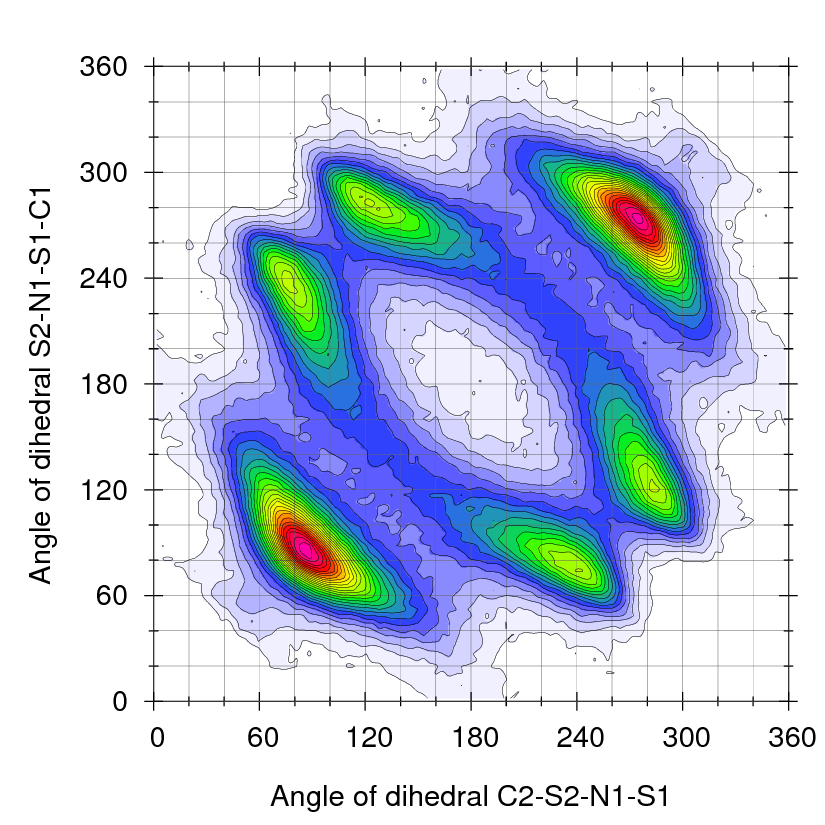
\includegraphics[width=\linewidth]{Ludwig_anion}
\caption{Combined distribution function of the dihedral angles of the contiguous chains C1-S1-N1-S2 and S1-N1-S2-C2 of anion \ce{[NTf_2]^-}, obtained from NPT-MD simulations of 250 ion pairs of \ce{[emim][NTf_2]} using the model of K\"{o}ddermann \textit{et al}. \cite{Koddermann_2007}.}
\label{fig:die_ntf2}
\end{figure}

\subsection{Dilute Solutions of \ce{CO_2} in \ce{[emim][B(CN)_4]} and \ce{[emim][NTf_2]}}
\label{sec:henry_results}

In Table \ref{table:henry}, we present results from expanded ensemble simulations of a single \ce{CO_2} molecule dissolved in 250 ion pairs of either \ce{[emim][B(CN)_4]} or \ce{[emim][NTf_2]} under periodic boundary conditions.
The simulations were carried out at $T = 298.0~\mathrm{K}$ and $P = 1.0~\mathrm{bar}$.
Table~\ref{table:henry} contains simulated molar densities, partial and total solvation free energies, as well as Henry's law constants ($K_s$) computed via Eq.~\eqref{eq:henry_eq}.
The uncertainties in $K_s$ were calculated by using a standard error propagation formula.
The computed values should be compared to the experimental data reported by Mahurin \textit{et al}. \cite{Mahurin_2010} ($K_s = 38.9 \pm 0.03 ~\mathrm{atm}$ for \ce{CO_2} in \ce{[emim][B(CN)_4]}) and by Finotello \textit{et al}. \cite{Finotello_2008} ($K_s = 39.0 \pm 0.1 ~\mathrm{atm}$ for \ce{CO_2} in \ce{[emim][NTf_2]}).

\begin{table*}
	\centering
	\caption{Results of solvation free energies and Henry's law constants of \ce{CO_2} in \ce{[emim][B(CN)_4]} and \ce{[emim][NTf_2]} at $T = 298.15~\mathrm{K}$ and $P = 1~\mathrm{atm}$. The experimental Henry constants of \ce{CO_2} in \ce{[emim][B(CN)_4]} and in \ce{[emim][NTf_2]} are, respectively, $38.9 \pm 0.03 ~\mathrm{atm}$ \cite{Mahurin_2010} and $39.0 \pm 0.1 ~\mathrm{atm}$ \cite{Finotello_2008}.}
	\begin{adjustbox}{max width=\textwidth}
		\begin{tabular}{ccccccc}  
			\hline\hline
			Model & $\tilde{\rho}_\text{sim}$ & $\Delta G_\text{vdW}$  & $\Delta G_\text{Coul}$  & $\Delta G_\text{sim}$ & $K_s$ & error \\
			& (mol/dm\textsuperscript{3}) & (kcal/mol) & (kcal/mol) &  (kcal/mol) & (atm)  & (\%) \\
			\hline
%			\multicolumn{7}{c}{\ce{[emim][B(CN)_4]}: $K_{s}^{\text{exp}} = 38.9 \pm 0.03 ~\mathrm{atm}$ \cite{Mahurin_2010}} \\
			\multicolumn{7}{c}{\ce{[emim][B(CN)_4]}} \\
			Koller \textit{et al}. \cite{Koller_2012} & $4.5925$ & $0.45 \pm 0.01$ & $-1.06 \pm 0.02$ & $-0.61 \pm 0.02$ & $40 \pm 1$ & $2.8$ \\
			Batista \textit{et al}. \cite{Batista_2015} & $4.3700$ & $0.378 \pm 0.008$ & $-1.24 \pm 0.01$  & $-0.86 \pm 0.01$ & $24.9 \pm 0.5$ & $38.9$ \\
			Liu \textit{et al}. \cite{Liu_2014} & $4.3815$ & $0.226 \pm 0.009$ & $-1.11 \pm 0.01$ & $-0.88 \pm 0.01$ & $24.3 \pm 0.5$ & $37.6$  \\
			Weber and Kirchner \cite{Weber_2016} & $4.5221$ & $0.478 \pm 0.009$ & $-1.23 \pm 0.02$ & $-0.75 \pm 0.02$ & $31 \pm 1$ & $20.3$  \\
			\hline
%			\multicolumn{7}{c}{\ce{[emim][NTf_2]}: $K_{s}^{\text{exp}} = 39.0 \pm 0.1 ~\mathrm{atm}$ \cite{Finotello_2008} }\\
			\multicolumn{7}{c}{\ce{[emim][NTf_2]}} \\
			K\"{o}ddermann \textit{et al}. \cite{Koddermann_2007} & $3.8205$ & $0.389 \pm 0.005$ & $-0.901 \pm 0.006$ & $-0.512 \pm 0.008$ & $39.4 \pm 0.5$  & $0.97$  \\
			\hline\hline
			\label{table:henry} 
		\end{tabular}
	\end{adjustbox}
\end{table*}

Is it worth remarking that the result of $\Delta G_\text{sim}$ obtained with the model of Liu \textit{et al}. \cite{Liu_2014} is statistically identical to a value reported by the same authors in Ref.~\citenum{Liu_2014_1}, where they applied the Bennett Acceptance Ratio (BAR) method \cite{Bennett_1976} to independent samples obtained with different values of $\lambda_\text{vdW}$ and $\lambda_\text{Coul}$.
Moreover, the $\Delta G_\text{sim}$ value we computed for \ce{[emim][NTf_2]} is very close to the one obtained by Kerl \textit{et al}. \cite{Kerl__2017} ($-0.534 ~\mathrm{kcal/mol}$, with no reported uncertainty) using the Free-Energy Perturbation (FEP) method \cite{Zwanzig_1954}.
%These consistencies have served for validating the methodological approaches of this work.

One can see in Table \ref{table:henry} that the only model able to reproduce the experimental Henry's law constant of \ce{CO_2} in \ce{[emim][B(CN)_4]} with small deviation is that of Koller \textit{et al}. \cite{Koller_2012}.
The worst results are obtained with the models of Batista \textit{et al}. \cite{Batista_2015} and Liu \textit{et al}. \cite{Liu_2014}.
These models fail in part because of the small values they predict for $\Delta G_\text{vdW}$.
In order to analyze the model distinctions in more detail, in Fig.~\ref{fig:deltag} we plot free energy profiles with respect to the coupling parameter $\lambda_\text{vdW}$, as obtained from the simulations with all \ce{[emim][B(CN)_4]} models.
We observe that the model of Batista \textit{et al}. \cite{Batista_2015} is the one that predicts the smallest free-energy barrier, immediately followed by the model of Liu \textit{et al}. \cite{Liu_2014}.
This observation suggests that these models underestimate the magnitude of the solvent-solvent interactions, thus making it easier to open a cavity in the system for inserting the solute.
Besides, it also explains why these models underestimate the density of \ce{[emim][B(CN)_4]}, such as seen in Table~\ref{table:props_dsf}.
The Liu \textit{et al}. \cite{Liu_2014} model predicts the smallest value of $\Delta G_\text{vdW}$ in spite of exhibiting only the second smallest free-energy barrier.
This occurs because the attractive van der Waals interactions compensate the cavity formation more favorably than in the case of Batista \textit{et al}. \cite{Batista_2015}, as one can observe in Fig.~\ref{fig:deltag} as $\lambda_\text{vdW}$ approaches unity.
Nevertheless, these distinctions end up being canceled out when the charges of the \ce{CO_2} molecule are introduced, since $\Delta G_\text{vdW}$ and $\Delta G_\text{Coul}$ sum up to very similar $\Delta G_\text{sim}$ results for both models.

\begin{figure}
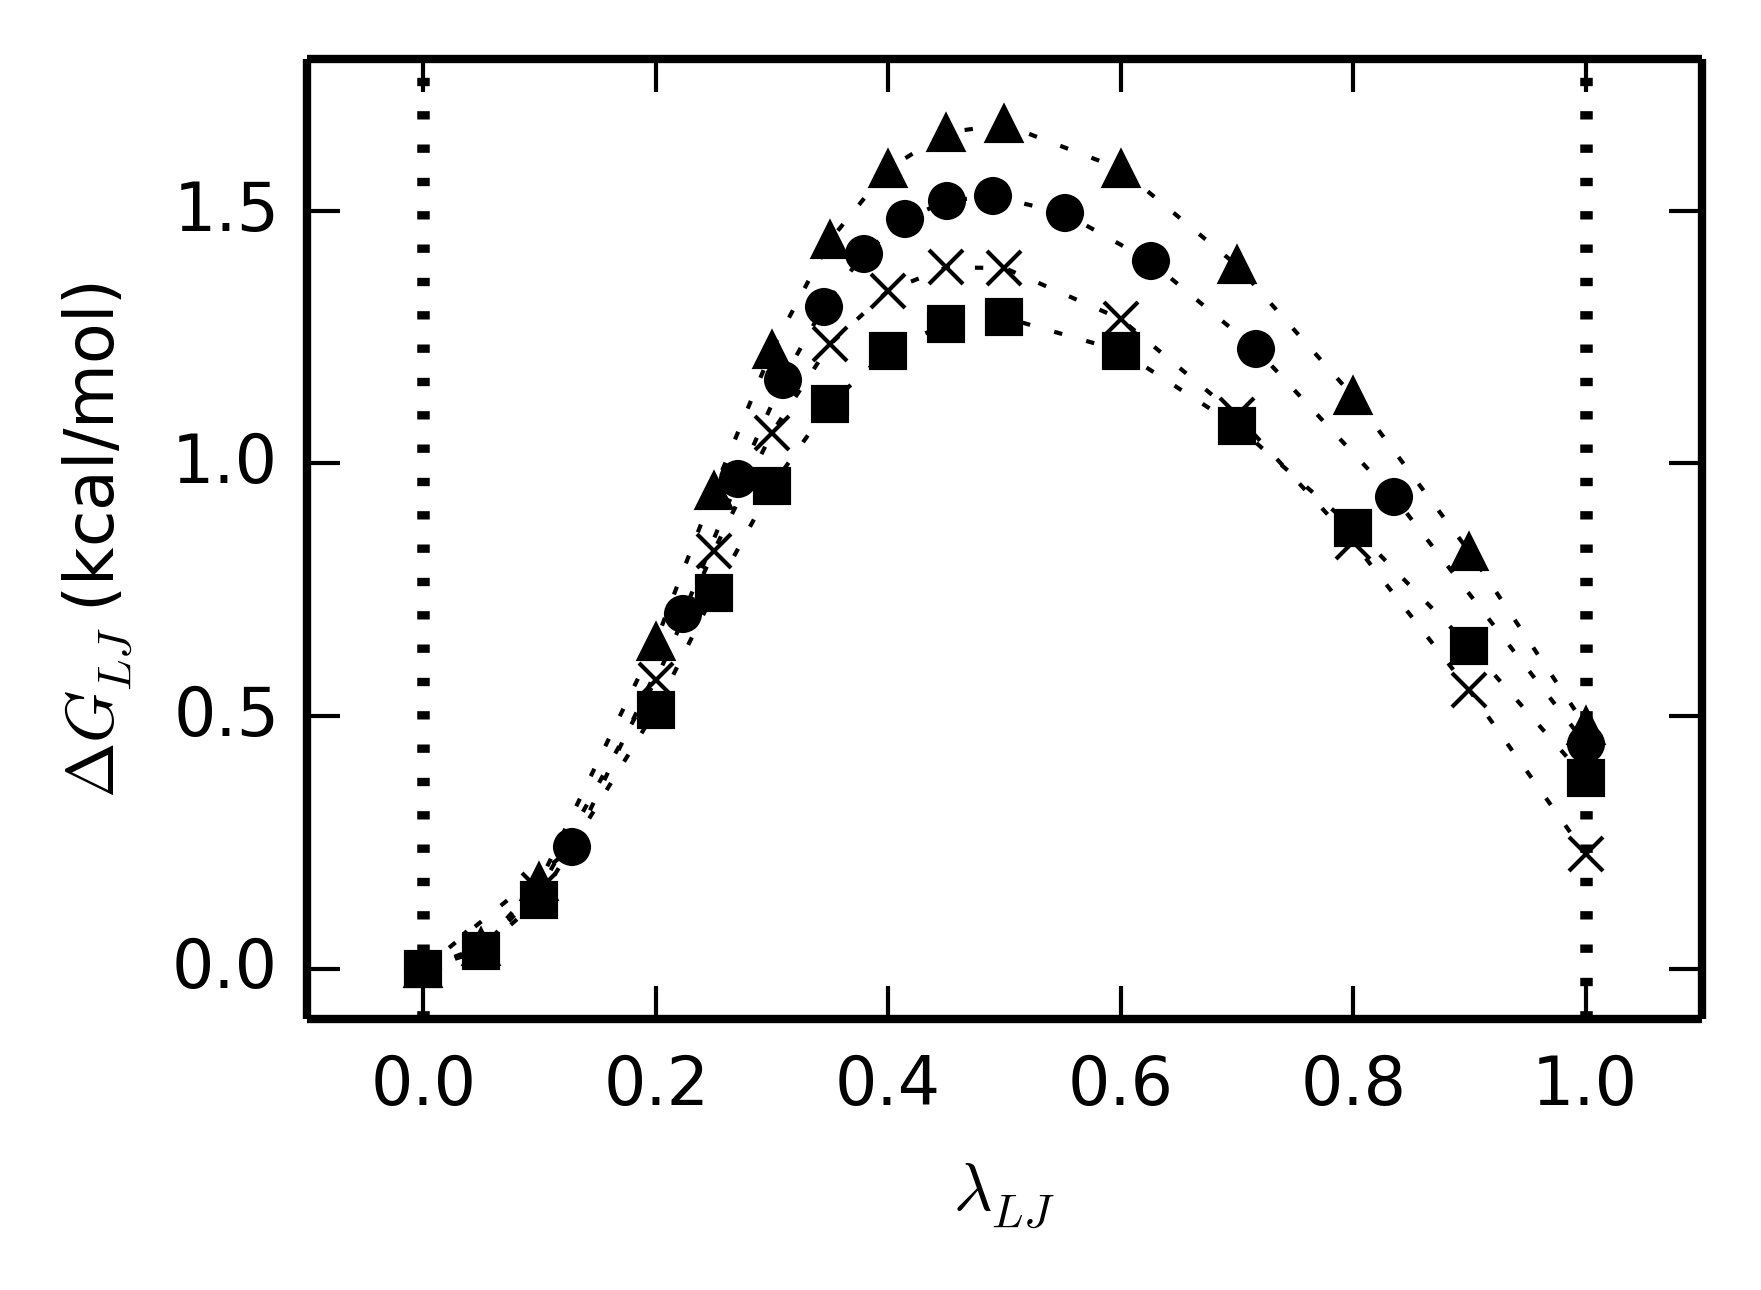
\includegraphics[width=\linewidth]{free_energy_paper}
\caption{Profile of $\Delta G_\text{vdW}$ corresponding to the insertion of a \ce{CO_2} molecule in \ce{[emim][B(CN)_4]}, modeled according to the force fields of Koller \textit{et al}. \cite{Koller_2012} ($\bullet$), Batista \textit{et al}. \cite{Batista_2015} ($\blacksquare$), Liu \textit{et al}. \cite{Liu_2014} ($\times$), and Weber and Kirchner \cite{Weber_2016} ($\blacktriangle$).}
\label{fig:deltag}
\end{figure}

Such as the model of Koller \textit{et al}. \cite{Koller_2012} does in the case of \ce{[emim][B(CN)_4]}, the one of K\"{o}ddermann \textit{et al}. \cite{Koddermann_2007} accurately predicts the Henry's law constant of \ce{CO_2} in \ce{[emim][NTf_2]}.
A comparison between the values of $\Delta G_\text{sim}$ obtained from these models, shown in Table \ref{table:henry}, suggests that the solvation of \ce{CO_2} takes place more favorably in \ce{[emim][B(CN)_4]} than in \ce{[emim][NTf_2]}.
The fact that $K_s$ has almost the same value in both cases is due to a compensation promoted by the distinct molar densities of these ionic liquids.
Spatial distribution functions (SDFs) \cite{Svishchev_1993} can help us visualizing how differently the solvent ions interact with the solute molecule.
By using TRAVIS \cite{Brehm_2011}, we have obtained SDFs of both cation and anion around a \ce{CO_2} molecule, sampled from MD trajectories of either \ce{CO_2}+\ce{[emim][B(CN)_4]} or \ce{CO_2}+\ce{[emim][NTf_2]} systems simulated at $T = 298.0~\text{K}$, $P = 1.0~\mathrm{bar}$, and $x_\mathrm{CO_2} = 0.1$.
The slightly larger \ce{CO_2} concentration considered here is meant to improve statistics.
The obtained SDFs were depicted as isosurfaces using VMD \cite{HUMP96}, with isovalues determined so as to highlight the first solvation shell.
The resulting images are shown in Fig.~\ref{fig:sdf_ions}.
By comparing Figs.~\ref{fig:sdf_ions}(a) and \ref{fig:sdf_ions}(b), we note that the gap between the regions occupied by the anion and the cation is smaller in the case of \ce{[emim][B(CN)_4]}.
In addition, the first solvation shell corresponding to \ce{[B(CN)_4]^-} occurs at a slightly shorter distance than that corresponding to \ce{[NTf_2]^-}, as one can clearly see by a direct comparison done in Fig.~\ref{fig:sdf_ions}(c).
This is in part due to the difference in size of these two anions.
The result is a higher density of negative charges around the carbon atom of \ce{CO_2}, whose point-charge is positive as a consequence of the oxygen's high electronegativity.
This seems to induce a greater stability of \ce{CO_2} when solvated in \ce{[emim][B(CN)_4]}, rather than in \ce{[emim][NTf_2]}, possibly resulting in enhanced solubility.
However, the mentioned similarity in the Henry's law constants could cause such enhancement to go unnoticed.
This makes clear the importance of carrying out a study at high \ce{CO_2} concentrations.

\begin{figure*}
\centering
\subfloat[]{%
  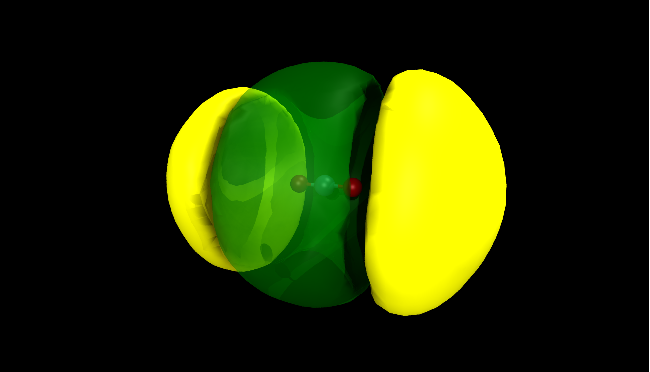
\includegraphics[width=\linewidth/3,trim={2cm 0 1.5cm 0},clip]{kollerall.pdf}
}
\subfloat[]{%
  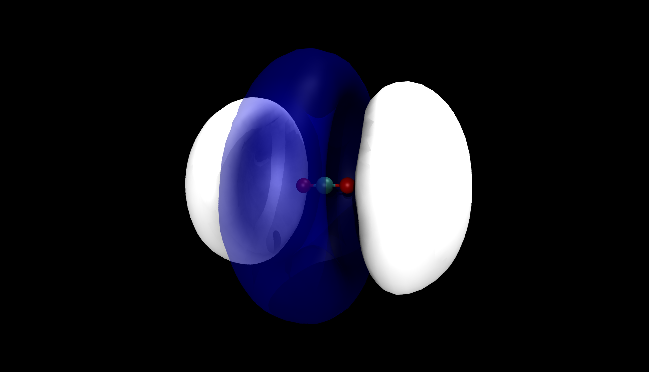
\includegraphics[width=\linewidth/3,trim={1.75cm 0 1.75cm 0},clip]{ludwigall.pdf}
}
\subfloat[]{%
  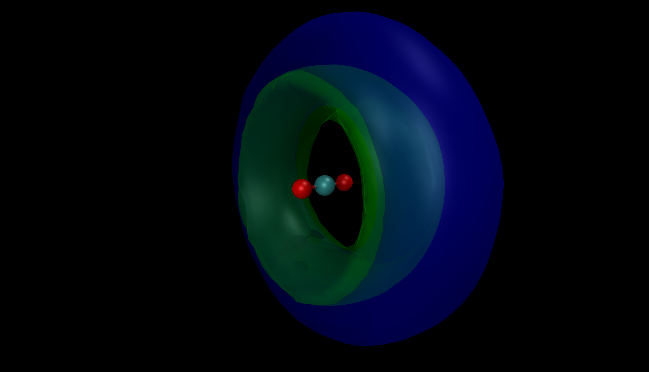
\includegraphics[width=\linewidth/3,trim={2.5cm 0 1cm 0},clip]{anionanion.pdf}
}
\caption{Spatial distribution functions (SDFs) of (a) \ce{[B(CN)_4]^-} (green) and \ce{[emim]^+} (yellow) at the isosurface values of 0.138 and 0.12, respectively; and of (b) \ce{[NTf_2]^-} (blue) and \ce{[emim]^+} (white) at the isosurface values of 0.086 and 0.063, respectively.
Fig. (c) corresponds to the SDFs of the anions plotted together.}
\label{fig:sdf_ions}
\end{figure*}

\subsection{Concentrated solutions of \ce{CO_2} in \ce{[emim][B(CN)_4]} and \ce{[emim][NTf_2]}}
\label{sec:results_conc}

Since concentrated solutions are the more likely scenario in carbon capture processes, we have also carried out simulations of systems with higher \ce{CO_2} concentrations.
The thermodynamic conditions specified for these simulations, which are based on experimental investigations \cite{Makino_2014,Schilderman_2007}, are shown in Table~\ref{table:solv}.
We have selected these specific conditions because of the proximity observed in the molality of \ce{CO_2} ($m_s$).
It is worth noting that the marked difference in the molar fractions of \ce{CO_2} in Table~\ref{table:solv} does not imply that \ce{[emim][NTf_2]} is a better solvent than \ce{[emim][B(CN)_4]}, thus exemplifying the observation made by Carvalho \textit{et al}. \cite{Carvalho_2016} and discussed here in Sec.~\ref{sec:intro}.

\begin{table}
	\centering
	\caption{Thermodynamic conditions, based on the experimental observations of Refs.~\citenum{Makino_2014} and \citenum{Schilderman_2007}, employed in the solvation study at high concentrations of \ce{CO_2} in \ce{[emim][B(CN)_4]} and \ce{[emim][NTf_2]}, as well as the results obtained via expanded ensemble simulations.}
	\begin{tabular}{ccc}
		\hline\hline
		IL & \ce{[emim][B(CN)_4]}  & \ce{[emim][NTf_2]} \\
		\hline
%		model & Ref.~\citenum{Koller_2012} & Ref.~\citenum{Koddermann_2007} \\
		\multicolumn{3}{c}{Specification} \\
		$T$  & $313.15~\mathrm{K}$ & $312.13~\mathrm{K}$ \\
		$P$  & $21~\mathrm{atm}$ & $37~\mathrm{atm}$ \\
		$x_s$ & $0.352$ & $0.479$ \\
		$m_s$ & $2.4~\mathrm{mol/kg}$ & $2.35~\mathrm{mol/kg}$ \\
		\hline
		\multicolumn{3}{c}{Simulation Result} \\
		$c_s$ & $3.04~\mathrm{mol/dm^3}$ & $2.22~\mathrm{mol/dm^3}$ \\ 
		$\Delta G_\text{sim}$ & $-0.755~\mathrm{kcal/mol}$ & $-0.542~\mathrm{kcal/mol}$ \\
		$P$ & $18.3~\mathrm{atm}$ & $38.4~\mathrm{atm}$ \\
		\hline\hline
		\label{table:solv} 
	\end{tabular}
\end{table}

We carried out expanded ensemble simulations of liquid solutions at the conditions of Table~\ref{table:solv}.
The model of Koller \textit{et al}. \cite{Koller_2012} was the one employed for simulating \ce{[emim][B(CN)_4]}.
The computed solvation free energies for the systems \ce{CO_2}+\ce{[emim][B(CN)_4]} and \ce{CO_2}+\ce{[emim][NTf_2]} were $-0.755 \pm 0.009 ~\mathrm{kcal/mol}$ and $-0.542 \pm 0.005~\mathrm{kcal/mol}$, respectively.
In Fig.~\ref{fig:pressure}, we present our predictions of the equilibrium pressure ($P$) obtained by solving Eq.~\eqref{eq:equilibrium pressure}, as well as the corresponding gas-phase fugacities of \ce{CO_2} ($f_s^g$) computed by Eq.~\eqref{eq:fgas_d}.
The dotted lines correspond to the experimental values (i.e. those used to simulate the liquid solutions).
First, the results make clear that assuming ideal gas ($P = f_s^g$) would have been an oversimplification, specially in the case of \ce{[emim][NTf_2]}.
Second, and most importantly, the computed pressures did not depart considerably from the specified values, meaning that our results sustain the experimental observations.
Therefore, as the pressure required to reach the same equilibrium molal concentration of \ce{CO_2} in the liquid phase is smaller for \ce{[emim][B(CN)_4]} than for \ce{[emim][NTf_2]}, our results confirm that the former is a better solvent than the latter.
This confirmation was possible by simulating a purely physical absorption, without considering any quantum effect.

\begin{figure}
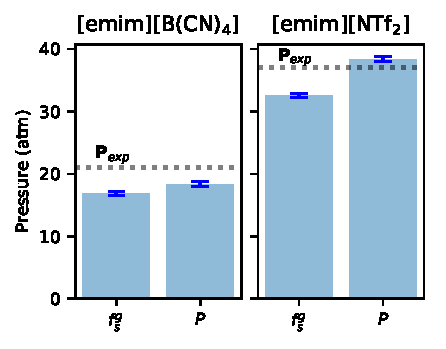
\includegraphics[width=\linewidth]{pressure_est.pdf}
\caption{Prediction of the gas-phase fugacity and partial pressure of \ce{CO_2} for the systems \ce{CO_2}-\ce{[emim][B(CN)_4]} and \ce{[emim][NTf_2]}.}
\label{fig:pressure}
\end{figure}

\subsection{Infinite-dilution activity coefficients in \ce{[emim][B(CN)_4]}}
\label{sec:act_results}

Having selected the model of \ce{[emim][B(CN)_4]} that best reproduces the experimental $K_s$ of \ce{CO_2}, we next calculate the infinite-dilution activity coefficients ($\gamma^{\, \infty}$) of benzene, hexane, cyclohexane, ethanol and water in \ce{[emim][B(CN)_4]}.

The task of accurately predicting $\gamma^{\, \infty}$ is challenging since, according to Eq.~\eqref{eq:gamma_inf}, one should reproduce the solvation free energies in both the pure solute and the solvent.
In Table~\ref{table:mu_solutes} we show the simulated densities and the solvation free energies $(\Delta G^{0}_\text{sim})$ of the pure solutes, which we compare against the experimental data extracted from the work of Chang~\cite{Chang_2009}.
It should be pointed out that we were unable to find the experimental $\Delta G^{0}_\text{exp}$ for cyclohexane.
Note that only in the case of ethanol we successfully predicted the $\Delta G^{0}_\text{exp}$.
The relative errors for the other solutes are around 10\%.

The results of $\gamma^{\, \infty}$ are presented in Table~\ref{table:gamma}.
For benzene and water, the predictions are very accurate, but this may be due to fortuitous error compensations given the divergences shown in Table~\ref{table:mu_solutes}.
From Table \ref{table:gamma}, one sees that the experimental $\gamma^{\, \infty}$ for hexane at $298.15~\text{K}$ and $303~\text{K}$ considerably differ.
It is therefore difficult to assess the reliability of our results in this case.

\begin{table*}
	\centering
	\caption{Solvation free energy at $T = 298.15~\text{K}$ for the pure solutes benzene, hexane, cyclohexane, ethanol and water.}
	\begin{adjustbox}{max width=\textwidth}
		\begin{tabular}{ccccccccc}
			\hline\hline
			Solute & $\rho_\text{sim}$ & error & $\Delta G_\text{vdW}$  & $\Delta G_\text{Coul}$  & $\Delta G^0_\text{sim}$ & $\Delta G^0_\text{exp}$   & error \\
			& (g/cm\textsuperscript{3}) & (\%) & (kcal/mol) &  (kcal/mol) &  (kcal/mol)   & (kcal/mol)   & (\%) \\
			\hline
			hexane & $0.6513 \pm 0.0003$ & $0.5$ & $-3.67  \pm  0.03$ & $0.011 \pm 0.007$ & $-3.66 \pm 0.03$ & $-4.06$ & $9.90$ \\
			cyclohexane & $0.7692 \pm 0.0007$ & $0.6$ & $-4.39 \pm 0.01$ & $0$ & $-4.39 \pm 0.01$ & n/a & n/a  \\
			benzene & $0.8611 \pm 0.0002$ & $1.4$ & $-3.75  \pm 0.02$ & $-0.381 \pm 0.007$ & $-4.14 \pm 0.02$ & $-4.56$ & $9.32$  \\
			ethanol & $0.781 \pm 0.008$ & $1.01$  & $-0.93 \pm 0.01$ & $-4.15 \pm 0.02$  & $-5.08  \pm 0.02$  & $-5.08$ & $0$ \\
			water & $0.9948 \pm 0.0003$ & $0.2$ & $2.015 \pm 0.004$ & $-9.01 \pm 0.02$ & $-6.99 \pm 0.02$ & $-6.33$  & $10.43$ \\
			\hline\hline
			\label{table:mu_solutes} 
		\end{tabular}
	\end{adjustbox}
\end{table*}

\begin{table*}
	\centering
	\caption{Infinite-dilution activity coefficients in \ce{[emim][B(CN)_4]} at $T = 298.15~\text{K}$ of the pure solutes benzene, hexane, cyclohexane, ethanol, and water.}
	\begin{adjustbox}{width=1\textwidth}
		\begin{tabular}{cccccccc}  
			\hline\hline
			Solute & $\Delta G_\text{vdW}$  & $\Delta G_\text{Coul}$  & $\Delta G_\text{sim}$  & $\gamma^\infty_\text{sim}$ & $\gamma^\infty_\text{exp}$ \cite{Doma_ska_2011} & $\gamma^\infty_\text{exp}$ \cite{Yan_2010} \\
			& (kcal/mol) & (kcal/mol) &  (kcal/mol)  & (298 K) & (298 K)  & (303 K) \\
			\hline
			hexane & $-2.13 \pm 0.04$ & $-0.152 \pm 0.007$ & $-2.282 \pm 0.04$ & $6.2 \pm 0.5$ & $33.8$ & $20.97$  \\
			cyclohexane & $-2.75 \pm 0.06$ & 0 & $-2.75 \pm 0.06$ & $9 \pm 1$ & $16.7$ & $13.82$ \\
			benzene & $-2.23 \pm 0.05$ & $-1.29 \pm 0.04$ & $-3.52 \pm 0.06$ & $1.2 \pm 0.1$ & $1.13$ & $1.31$ \\ 
			ethanol & $-0.73 \pm 0.02$ & $-4.10 \pm 0.04$ & $-4.83 \pm 0.04$ & $0.41 \pm 0.03$ & $1.58$ & $1.64$  \\
			water & $1.38 \pm 0.008$ & $-6.32 \pm 0.03$ & $-4.94 \pm 0.03$ & $2 \pm 1$ & $2.65$ & $2.24$ \\
			\hline\hline
			\label{table:gamma} 
		\end{tabular}
	\end{adjustbox}
\end{table*}

\section{Concluding remarks}
\label{sec:conclusion}

One of the goals of this paper was to compare various available models of \ce{[emim][B(CN)_4]} in terms of their capability to reproduce the experimental Henry constant of \ce{CO_2}.
We have found that only the force field developed by Koller \textit{et al}. \cite{Koller_2012} is able to perform such task, with a small relative error of 2.8 \%.
A key factor for its success seems to be the reparametrization of the LJ parameters for the boron atom carried out in that work, which also allows to accurately reproduce the experimental density of the pure substance.

We focused also on exploring alternative simulation strategies with the goal of gaining computational efficiency.
Particularly, for both \ce{[emim][B(CN)_4]} and \ce{[emim][NTf_2]}, we concluded that the DSF method with $\alpha$ = 0.2 {\AA}$^{-1}$ is a suitable strategy.
Other improvement was the use of rigid bodies to simulate \ce{[emim][B(CN)_4]}.
This required preliminary simulations in order to examine the flexibility of the ethyl chain in \ce{[emim]^+} and the analysis was greatly facilitated by employing useful visualization tools.
Besides the properties already mentioned, the different models showed quite different behaviors, as well.
This lack of consistency is one of the reasons why in industry molecular simulation has not become a routinely tool yet.

The solvation free energy results at infinite-dilution condition suggest a slightly more favorable solvation of \ce{CO_2} in \ce{[emim][B(CN)_4]} than in  \ce{[emim][NTf_2]}.
However, this picture changes at high concentrations: the simulations correctly predicted a considerable lower pressure to dissolve a certain mass of \ce{CO_2} in \ce{[emim][B(CN)_4]}.

Finally, we employed the model of Koller \textit{et al}. \cite{Koller_2012} to predict infinite-dilution activity coefficients of various solutes.
In this case, the results were not satisfactory given the large errors in the free energy calculations of the pure solutes, making necessary a revision of their force fields in a future work.

\section*{Acknowledgments}
The authors acknowledge the financial support provided by Petrobras (project code CENPES 16113). 

\section*{References}

\bibliography{ionic_liquids}

\end{document}